% Copyright 2026 Sreeram Anil
% SPDX-License-Identifier: CC-BY-4.0
% =============================================================================
%  Multiplicative extended Kalman filter — attitude (AHRS) family
% =============================================================================
\chapter{Multiplicative Extended Kalman Filter (MEKF)}
\label{ch:att-mekf}

\section*{At a glance}
\begin{tabular}{@{}l>{\raggedright\arraybackslash}p{0.76\textwidth}@{}}
Family & attitude / AHRS \\
Header & \texttt{include/estkit/attitude/mekf.hpp} \\
Registered name & \texttt{MEKF} \\
State & $\hat{\bm{q}}\in S^3$, $\hat{\bm{b}}\in\real^3$; error
 $[\delta\bm{\theta};\delta\bm{b}]\in\real^6$, $\mP\in\real^{6\times6}$ \\
Cost per step & $\approx2.9\times10^3$ MACs; $\SI{2.04}{\micro\second}$/step, 608\,bytes \\
Primary references & \cite{lefferts1982,markley2003mekf,crassidis2007survey,farrenkopf1978,bucyjoseph1968} \\
\end{tabular}

\section{Motivation and aerospace relevance}
Attitude is the canonical example of a state that does not live in a vector space. A quaternion has
four components and three degrees of freedom; an ordinary EKF that carries a $4\times4$ covariance
for it is describing a distribution on $\real^4$ whose support is a three-dimensional sphere, so
$\mP$ is necessarily singular in the radial direction and the filter must fight the norm constraint
at every step. Lefferts, Markley and Shuster~\cite{lefferts1982} settled the matter for spacecraft
in 1982: keep the quaternion as a \emph{reference} that carries the large, nonlinear part of the
attitude, and let the Kalman filter estimate only a small three-parameter \emph{error} that is
composed with it multiplicatively. The covariance is then a genuine $3\times3$ (or, with the gyro
bias, $6\times6$) object with no constraint attached.

Markley~\cite{markley2003mekf} showed that all the usual three-parameter error representations ---
rotation vector, Gibbs vector, modified Rodrigues parameters, the quaternion vector part --- agree
to second order and differ only in how the reset step is implemented, so the choice is a matter of
taste rather than accuracy. Crassidis, Markley and Cheng~\cite{crassidis2007survey} survey what came
afterwards, of which the unscented variant~\cite{crassidismarkley2003} is the closest relative;
the MEKF remains the reference against which everything is compared, and it flies on
essentially every spacecraft and every high-grade AHRS.

For a battery-management toolbox the MEKF is the aerospace half of the same idea that makes the
error-state formulation attractive in Chapter~\ref{ch:ekf}: linearise the \emph{deviation}, not the
state, so that the operating point never has to be re-derived.

\section{Problem statement and assumptions}
Conventions as in Chapter~\ref{ch:att-complementary}; $\bm{R}$ denotes a rotation and measurement
covariances are written $\bm{\Sigma}$.

\paragraph{Process model.} The gyro is treated as an \emph{input}, not as a measurement of a
dynamic model --- there is no vehicle model at all. With the Farrenkopf~\cite{farrenkopf1978} gyro
error model,
\begin{equation}
\bm{\omega}_y = \bm{\omega} + \bm{b} + \bm{n}_v,\qquad
\dot{\bm{b}} = \bm{n}_u,\qquad
\bm{n}_v\sim\N{\bm{0}}{\sigma_v^2\bm{I}\,\delta(t-\tau)},\quad
\bm{n}_u\sim\N{\bm{0}}{\sigma_u^2\bm{I}\,\delta(t-\tau)} ,
\label{eq:mekf-gyro}
\end{equation}
$\sigma_v$ is the angle random walk (rad\,s$^{-1/2}$) and $\sigma_u$ the rate random walk
(rad\,s$^{-3/2}$). The attitude obeys $\dot{\bm{q}}=\tfrac12\bm{q}\otimes[0,\bm{\omega}]$.

\paragraph{Measurement model.} Any body-frame observation of a known NAV vector $\bm{r}$,
\begin{equation}
\bm{y} = \bm{R}^\T\bm{r} + \bm{n},\qquad \bm{n}\sim\N{\bm{0}}{\bm{\Sigma}} .
\label{eq:mekf-meas}
\end{equation}
Two are used: $\bm{r}_a=[0,0,-g]^\T$ with $\bm{y}=\bm{f}$, and $\bm{r}_m=\bm{m}_{\text{nav}}$ with
$\bm{y}=\bm{m}$.

\paragraph{The multiplicative error.} Define
\begin{equation}
\bm{q} = \hat{\bm{q}}\otimes\exp(\delta\bm{\theta}),\qquad
\bm{b} = \hat{\bm{b}} + \delta\bm{b},\qquad
\bm{x} = \begin{bmatrix}\delta\bm{\theta}\\ \delta\bm{b}\end{bmatrix}\in\real^6,\qquad
\bm{x}\sim\N{\bm{0}}{\mP} .
\label{eq:mekf-err}
\end{equation}
$\delta\bm{\theta}$ is a BODY-frame rotation vector. Between updates $\bm{x}\equiv\bm{0}$ by
construction (the reset of \S\ref{sec:mekf-reset} pushes every correction into
$\hat{\bm{q}},\hat{\bm{b}}$), so the three-parameter representation never has to describe a large
rotation and $\mP$ never becomes singular.

\section{Derivation}

\subsection{Error kinematics}
Let $\hat{\bm{\omega}}=\bm{\omega}_y-\hat{\bm{b}}$ be the estimated rate. Write
$\delta\bm{q}=\hat{\bm{q}}^*\otimes\bm{q}$ and differentiate:
\begin{equation}
\dot{\delta\bm{q}} = \dot{\hat{\bm{q}}}^*\otimes\bm{q} + \hat{\bm{q}}^*\otimes\dot{\bm{q}}
 = \tfrac12\big(\delta\bm{q}\otimes[0,\bm{\omega}] - [0,\hat{\bm{\omega}}]\otimes\delta\bm{q}\big).
\label{eq:mekf-dq}
\end{equation}
Substituting $\delta\bm{q}=[1,\tfrac12\delta\bm{\theta}]+O(\norm{\delta\bm{\theta}}^2)$ and
$\bm{\omega}=\hat{\bm{\omega}}+\Delta\bm{\omega}$, the scalar parts cancel and the vector part of
\eqref{eq:mekf-dq} gives
\begin{equation}
\dot{\delta\bm{\theta}} = -\hat{\bm{\omega}}\times\delta\bm{\theta} + \Delta\bm{\omega}
 = -[\hat{\bm{\omega}}]_\times\,\delta\bm{\theta} - \delta\bm{b} - \bm{n}_v ,
\label{eq:mekf-dtheta}
\end{equation}
because $\Delta\bm{\omega}=\bm{\omega}-\hat{\bm{\omega}}
=(\bm{\omega}_y-\bm{b}-\bm{n}_v)-(\bm{\omega}_y-\hat{\bm{b}})=-\delta\bm{b}-\bm{n}_v$. Together with
$\dot{\delta\bm{b}}=\bm{n}_u$,
\begin{equation}
\dot{\bm{x}} = \mF\bm{x} + \mG\bm{n},\qquad
\mF=\begin{bmatrix}-[\hat{\bm{\omega}}]_\times & -\bm{I}\\ \bm{0}&\bm{0}\end{bmatrix},\qquad
\mG=\begin{bmatrix}-\bm{I}&\bm{0}\\ \bm{0}&\bm{I}\end{bmatrix},\qquad
\bm{n}=\begin{bmatrix}\bm{n}_v\\ \bm{n}_u\end{bmatrix}.
\label{eq:mekf-F}
\end{equation}

\subsection{Discrete transition matrix}
$\mF$ is block upper triangular with a nilpotent lower-right block, and $[\hat{\bm{\omega}}]_\times$
is constant over one sample, so $\bm{\Phi}=\exp(\mF\dt)$ can be written in closed form. With
$\bm{a}=\hat{\bm{\omega}}\dt$, $\vartheta=\norm{\bm{a}}$,
\begin{align}
\bm{\Phi}_{11} &= \exp\!\big(-[\bm{a}]_\times\big)
 = \bm{I} - \frac{\sin\vartheta}{\vartheta}[\bm{a}]_\times
  + \frac{1-\cos\vartheta}{\vartheta^2}[\bm{a}]_\times^2 ,
 \label{eq:mekf-phi11}\\
\bm{\Phi}_{12} &= -\!\int_0^{\dt}\!\exp\!\big(-[\hat{\bm{\omega}}]_\times\tau\big)\,d\tau
 = -\dt\left(\bm{I} - \frac{1-\cos\vartheta}{\vartheta^2}[\bm{a}]_\times
  + \frac{\vartheta-\sin\vartheta}{\vartheta^3}[\bm{a}]_\times^2\right),
 \label{eq:mekf-phi12}
\end{align}
with $\bm{\Phi}_{21}=\bm{0}$, $\bm{\Phi}_{22}=\bm{I}$ (Lefferts et al.~\cite{lefferts1982},
Eq.~(2.9); Markley \& Crassidis~\cite{markleycrassidis2014}, Eq.~(6.60)). The series limits
$\sin\vartheta/\vartheta\to1$, $(1-\cos\vartheta)/\vartheta^2\to\tfrac12$,
$(\vartheta-\sin\vartheta)/\vartheta^3\to\tfrac16$ are used below $\vartheta=10^{-6}$.

\subsection{Discrete process noise (Farrenkopf's model)}
Van Loan's construction~\cite{vanloan1978} applied to \eqref{eq:mekf-F} with
$[\hat{\bm{\omega}}]_\times$ neglected inside the integral (its effect is $O(\vartheta^2)$ relative,
$<10^{-5}$ at $\SI{100}{\hertz}$) gives, with $\bm{\Phi}(\tau)=\big[\begin{smallmatrix}\bm{I}&-\tau\bm{I}\\ \bm{0}&\bm{I}\end{smallmatrix}\big]$,
\begin{equation}
\mQ_d=\int_0^{\dt}\bm{\Phi}(\tau)\,\mG\begin{bmatrix}\sigma_v^2\bm{I}&\\&\sigma_u^2\bm{I}\end{bmatrix}\mG^\T\bm{\Phi}(\tau)^\T d\tau
=\begin{bmatrix}
 \big(\sigma_v^2\dt+\tfrac13\sigma_u^2\dt^3\big)\bm{I} & -\tfrac12\sigma_u^2\dt^2\,\bm{I}\\[2pt]
 -\tfrac12\sigma_u^2\dt^2\,\bm{I} & \sigma_u^2\dt\,\bm{I}
\end{bmatrix},
\label{eq:mekf-Q}
\end{equation}
the classical Farrenkopf~\cite{farrenkopf1978} result. The negative cross-term is not cosmetic: it
encodes the fact that an over-estimated bias produces a \emph{negative} attitude drift, and dropping
it makes the filter optimistic about how quickly the bias becomes observable.

\paragraph{Units.} The benchmark configuration supplies \emph{per-sample} standard deviations: the
gyro noise is added once per sample with standard deviation $\sigma_d$, and the bias increment once
per sample with standard deviation $\sigma_{rw}$. The angle accumulated from gyro noise in one step
is $\sigma_d\dt$, and \eqref{eq:mekf-Q} says it is $\sigma_v\sqrt{\dt}$; the bias increment is
$\sigma_u\sqrt{\dt}$. Hence
\begin{equation}
\sigma_v = \sigma_d\sqrt{\dt},\qquad \sigma_u = \sigma_{rw}/\sqrt{\dt} ,
\label{eq:mekf-units}
\end{equation}
which for the nominal scenario gives
$\sigma_v = \SI{1.75e-3}{\radian\per\second}\times0.1 = \SI{1.75e-4}{}$ and
$\sigma_u=\SI{3.49e-5}{}\times10=\SI{3.49e-4}{}$ in SI units. Getting
\eqref{eq:mekf-units} wrong by the factor $\dt$ is the single most common error in AHRS tuning; it
scales $\mQ$ by $10^4$ here.

\subsection{Measurement Jacobian}
From $\bm{R}(\hat{\bm{q}}\otimes\exp(\delta\bm{\theta}))=\hat{\bm{R}}\exp([\delta\bm{\theta}]_\times)
\approx\hat{\bm{R}}(\bm{I}+[\delta\bm{\theta}]_\times)$ we get
$\bm{R}^\T\approx(\bm{I}-[\delta\bm{\theta}]_\times)\hat{\bm{R}}^\T$, hence for \eqref{eq:mekf-meas}
\begin{equation}
\bm{y} \approx \hat{\bm{R}}^\T\bm{r} - \delta\bm{\theta}\times(\hat{\bm{R}}^\T\bm{r}) + \bm{n}
 = \underbrace{\hat{\bm{R}}^\T\bm{r}}_{\hat{\bm{y}}}
  + \underbrace{\big[\hat{\bm{R}}^\T\bm{r}\big]_\times}_{\mH_{\delta\theta}}\delta\bm{\theta} + \bm{n},
\qquad
\mH = \big[\;[\hat{\bm{R}}^\T\bm{r}]_\times \;\;\bm{0}_{3\times3}\;\big] .
\label{eq:mekf-H}
\end{equation}
$\mH$ has rank 2: a rotation about $\hat{\bm{R}}^\T\bm{r}$ leaves the observation unchanged, which
is why a single vector observation can never fix the attitude. Two non-collinear observations give
$\mH\in\real^{6\times6}$ of rank 3 in the attitude block and the attitude becomes observable
instantaneously; the bias block is observable only through the coupling $\bm{\Phi}_{12}$, i.e. over
time.

\subsection{Update and reset}\label{sec:mekf-reset}
Stacking the accelerometer and magnetometer blocks, the update is the textbook one about the
\emph{zero} prior error state:
\begin{align}
\bm{z} &= \begin{bmatrix}\bm{f}-\hat{\bm{R}}^\T\bm{r}_a\\ \bm{m}-\hat{\bm{R}}^\T\bm{r}_m\end{bmatrix},
\qquad
\mS = \mH\mP\mH^\T+\bm{\Sigma},\qquad \mK=\mP\mH^\T\mS\inv,\label{eq:mekf-K}\\
\bm{x}^+ &= \mK\bm{z},\qquad
\Pplus = (\mI-\mK\mH)\Pminus(\mI-\mK\mH)^\T + \mK\bm{\Sigma}\mK^\T ,\label{eq:mekf-P}
\end{align}
the Joseph form~\cite{bucyjoseph1968}, followed immediately by the \emph{reset} that returns the
error state to zero (Markley~\cite{markley2003mekf}, Sec.~V):
\begin{equation}
\hat{\bm{q}} \leftarrow \hat{\bm{q}}\otimes\exp\!\big(\delta\bm{\theta}^+\big),\qquad
\hat{\bm{b}} \leftarrow \hat{\bm{b}} + \delta\bm{b}^+,\qquad
\bm{x}\leftarrow\bm{0} .
\label{eq:mekf-reset}
\end{equation}
The reset is what makes the filter \emph{multiplicative}: the large rotation is absorbed by a
quaternion product, which is exact, and only the residual --- now zero --- is carried in the linear
state. To first order the reset leaves $\mP$ unchanged; the second-order correction
$\Pplus_{11}\leftarrow(\bm{I}-\tfrac12[\delta\bm{\theta}^+]_\times)\Pplus_{11}(\cdot)^\T$ is
$O(\norm{\delta\bm{\theta}^+}^2)$ and, as in every standard implementation, omitted.

\subsection{Measurement covariance: the part that is not textbook}
\label{sec:mekf-R}
For an AHRS the sensor noise is not the dominant error of \eqref{eq:mekf-meas} --- the \emph{model}
is. The accelerometer measures $\bm{R}^\T(\bm{a}_{\text{nav}}-\bm{g}_{\text{nav}})$ and the filter
pretends it measures $-\bm{R}^\T\bm{g}_{\text{nav}}$; the magnetometer sees hard-iron and local
field errors. $\bm{\Sigma}$ is therefore built as
\begin{equation}
\bm{\Sigma}_a = \big(\sigma_a^2+\sigma_{a,\text{extra}}^2+\sigma_{x,a}^2\big)\bm{I},\qquad
\bm{\Sigma}_m = \big(\sigma_m^2+\sigma_{m,\text{extra}}^2+\sigma_{x,m}^2\big)\bm{I},
\label{eq:mekf-R}
\end{equation}
with the disturbance terms
\begin{equation}
\sigma_{x,a} = \sqrt{\big(k_a\,e_a\big)^2 + \big(V_{\text{ref}}\max(0,\norm{\bm{\omega}_{yz}}-\varpi)\big)^2},
\qquad
\sigma_{x,m} = k_m\,e_m ,
\label{eq:mekf-sx}
\end{equation}
where $e_a,e_m$ are the low-pass-filtered magnitude anomalies of \eqref{eq:cf-weight} and
$\bm{\omega}_{yz}$ is the $(y,z)$ part of the bias-compensated rate.

The second term of $\sigma_{x,a}$ deserves its own statement, because a magnitude check alone does
\emph{not} work.
\begin{remark}[A coordinated turn is invisible to a norm test]\label{rem:mekf-turn}
In a coordinated turn at bank $\phi$ the specific force stays aligned with the body $z$ axis and has
magnitude $g/\cos\phi$. At $\phi=25^\circ$ that is $1.10\,g$: the \emph{direction} is wrong by
$25^\circ$ while the \emph{magnitude} is wrong by $10\,\%$, i.e. by
$\SI{1}{\metre\per\second\squared}$, comparable to ordinary turbulence. What does reveal the
condition is the rate: from $\bm{f}=\dot{\bm{v}}_b+\bm{\omega}\times\bm{v}_b-\bm{R}^\T\bm{g}$ the
unmodelled part is bounded by $\norm{\bm{\omega}\times\bm{v}_b}=V\norm{\bm{\omega}_{yz}}$ for an
aircraft flying along its $x$ axis. Bounding $V$ by the airframe's nominal airspeed
$V_{\text{ref}}$ --- a design constant, not a measurement --- gives a rate-driven standard deviation
that inflates $\bm{\Sigma}_a$ exactly when the aircraft manoeuvres. This is the covariance version
of the Euston et al.~\cite{euston2008} correction used in Chapter~\ref{ch:att-complementary}: it
widens the uncertainty instead of correcting the mean, and needs no airspeed sensor.
\end{remark}
The dead-zone $\varpi$ covers the residual rate uncertainty (bias plus noise). Without it an
uncompensated gyro bias would appear as a permanent manoeuvre and switch the accelerometer off for
ever --- a dead-lock, since the bias estimate needs the accelerometer.

Finally, and equally importantly, \eqref{eq:mekf-R} is capped by \emph{editing}: if
$\sigma_{x,a}$ exceeds a threshold, the accelerometer block is skipped entirely (formally
$\bm{\Sigma}_a\to\infty$), and likewise for the magnetometer. The reason is that a manoeuvre or a
magnetic anomaly is a \emph{systematic} error lasting thousands of samples, not white noise: with a
merely inflated but finite $\bm{\Sigma}$, the Kalman filter accumulates $N$ correlated samples and
converges to the biased answer with effective standard deviation $\sigma/\sqrt{N}$. Measurement
editing is the standard treatment (Gelb~\cite[Sec.~4.5]{gelb1974};
Tapley et al.~\cite[Sec.~4.15]{tapley2004}) and is worth a factor of $2.5$ here (results below).

\section{Algorithm}
\begin{algorithm}[H]
\caption{MEKF --- one sampling period}
\begin{algorithmic}[1]
\Require $\hat{\bm{q}},\hat{\bm{b}},\mP$; $\bm{\omega}_y,\bm{f},\bm{m}$; $\sigma_v,\sigma_u,\bm{\Sigma}$ parameters
\State \textbf{Time update:} $\hat{\bm{\omega}}\gets\bm{\omega}_y-\hat{\bm{b}}$;\;
       $\hat{\bm{q}}\gets\hat{\bm{q}}\otimes\exp(\hat{\bm{\omega}}\dt)$, normalise
\State $\bm{\Phi}\gets$ \eqref{eq:mekf-phi11}--\eqref{eq:mekf-phi12};\;
       $\mQ_d\gets$ \eqref{eq:mekf-Q};\;
       $\mP\gets\bm{\Phi}\mP\bm{\Phi}^\T+\mQ_d$; symmetrise
\State \textbf{Measurement update:} $\hat{\bm{y}}_a\gets\hat{\bm{R}}^\T\bm{r}_a$,\;
       $\hat{\bm{y}}_m\gets\hat{\bm{R}}^\T\bm{r}_m$
\State $\bm{\Sigma}\gets$ \eqref{eq:mekf-R}--\eqref{eq:mekf-sx}; \textbf{edit} blocks whose
       disturbance exceeds the threshold
\State $\mH\gets\big[\begin{smallmatrix}[\hat{\bm{y}}_a]_\times&\bm{0}\\ [\hat{\bm{y}}_m]_\times&\bm{0}\end{smallmatrix}\big]$;\;
       $\bm{z}\gets[\bm{f}-\hat{\bm{y}}_a;\;\bm{m}-\hat{\bm{y}}_m]$
\State $\mS\gets\mH\mP\mH^\T+\bm{\Sigma}$;\; $\mK\gets\mP\mH^\T\mS\inv$;\;
       \textbf{if} $\mK$ not finite \textbf{then return}
\State $\bm{x}^+\gets\mK\bm{z}$;\;
       $\mP\gets(\mI-\mK\mH)\mP(\mI-\mK\mH)^\T+\mK\bm{\Sigma}\mK^\T$; symmetrise
\State \textbf{Reset:} $\hat{\bm{q}}\gets\hat{\bm{q}}\otimes\exp(\delta\bm{\theta}^+)$, normalise;\;
       $\hat{\bm{b}}\gets\operatorname{clamp}(\hat{\bm{b}}+\delta\bm{b}^+)$
\Ensure $\hat{\bm{q}},\hat{\bm{b}},\mP$
\end{algorithmic}
\end{algorithm}

\section{Application to the benchmark flight}
$\mQ$ comes straight from the configuration through \eqref{eq:mekf-units}; nothing is tuned there
($q_{\text{scale}}=1$). $\mP_0=\diag\big((30^\circ)^2\bm{I},(\SI{3}{\degree\per\second})^2\bm{I}\big)$:
a $30^\circ$ initial attitude uncertainty is the standard ``unknown coarse alignment'' value and
covers the $46.6^\circ$ of the \texttt{init\_error} scenario, and
$\SI{3}{\degree\per\second}$ of bias uncertainty covers the \texttt{gyro\_bias} scenario.

Only $\bm{\Sigma}$ carries engineering judgement:
$\sigma_{a,\text{extra}}=\SI{0.5}{\metre\per\second\squared}$ (about $3^\circ$ of tilt) for the
residual linear acceleration of ordinary flight;
$\sigma_{m,\text{extra}}=\SI{1.5}{\micro\tesla}$ for the airframe's field-model error (a
deliberately conservative figure: the dataset's residual hard iron after calibration is only
$\SI{0.42}{\micro\tesla}$, and the registry comment quoting $\SI{1.37}{\micro\tesla}$ predates the
compass recalibration --- see the sensitivity study below, where the value turns out not to matter
on any scenario except \texttt{init\_error});
$V_{\text{ref}}=\SI{45}{\metre\per\second}$ (the nominal cruise airspeed) and
$\varpi=\SI{0.02}{\radian\per\second}$ for the manoeuvre bound; editing thresholds
$\SI{1}{\metre\per\second\squared}$ and $\SI{3}{\micro\tesla}$. The centripetal \emph{mean}
correction is available as an option but is switched \textbf{off}: see the results.

\section{Implementation notes}
Per step: $\bm{\Phi}\mP\bm{\Phi}^\T$ is $2\times216$ MACs, $\mH\mP\mH^\T$ another $432$, the
$6\times6$ LU inverse about $290$, $\mP\mH^\T\mS\inv$ $432$, and the Joseph form $1080$ --- about
$2.9\times10^3$ multiply--adds in total, plus two $3\times3$ rotation matrices and one quaternion
exponential. Measured $\SI{2.04}{\micro\second}$/step, 15 times the Mahony filter and
still three orders of magnitude inside the $\SI{10}{\milli\second}$ budget at $\SI{100}{\hertz}$; on
a $\SI{216}{\mega\hertz}$ Cortex-M7 in float32 this is of order $\SI{40}{\micro\second}$, i.e.
$0.4\,\%$ duty. \code{sizeof} is 608\,bytes, dominated by the $6\times6$ covariance (288\,B).

The right half of $\mH$ is structurally zero and both blocks are $3\times3$ skew matrices; a
hand-rolled version exploiting that, and doing two sequential $3$-dimensional updates instead of one
$6$-dimensional one, would cut the cost roughly in half and remove the $6\times6$ inverse. The
generic form was kept because it is what \code{linalg.hpp} expresses naturally and because the
sequential form is not algebraically identical when the two blocks are correlated through $\mP$.

Numerical hygiene: $\mP$ is symmetrised after both the time and the measurement update; the Joseph
form is used (\code{joseph=true}); the gain and the correction are checked with \code{is\_finite()}
and the update is skipped rather than propagating NaN; the quaternion is renormalised after the
reset; the bias is clamped to $\pm\SI{15}{\degree\per\second}$; $\bm{\Phi}$ falls back to its series
form below $\vartheta=10^{-6}$. Measured: \code{joseph=false} and \code{exact\_phi=false} both give
\emph{bit-identical} mission statistics here ($\SI{2.11}{\degree}$, seed~1), which says that at
$\SI{100}{\hertz}$ with $\norm{\bm{\omega}}\dt<10^{-3}$ neither the second-order terms of
\eqref{eq:mekf-phi11} nor the Joseph stabilisation is being exercised --- they are insurance, not
accuracy. The single-precision build reproduces the double-precision RMS to four digits.

\section{Benchmark results}
% Copyright 2026 Sreeram Anil
% SPDX-License-Identifier: CC-BY-4.0
\begin{table}[H]\centering\footnotesize\setlength{\tabcolsep}{3.5pt}\caption{MEKF: attitude benchmark (mean over seeds; all angles in degrees; $t_\mathrm{conv}$: first time the attitude error stays below 2$^\circ$ for 30\,s; bias RMSE in deg/s; 608 bytes of state).}\label{tab:imu_MEKF}
\begin{tabular}{lrrrrrrrrcr}\toprule scenario & RMS & roll & pitch & yaw & max & RMS$_\mathrm{ss}$ & $t_\mathrm{conv}$ [s] & bias RMSE & lost & ns/step \\ \midrule
nominal & 2.48 & 0.84 & 0.68 & 2.23 & 15.1 & 3.07 & 0 & 0.17 & no & 2037 \\
init\_error & 2.50 & 0.85 & 0.68 & 2.25 & 15.1 & 3.07 & 3 & 0.25 & no & 2039 \\
gyro\_bias & 2.48 & 0.84 & 0.68 & 2.23 & 15.1 & 3.07 & 2 & 0.19 & no & 2053 \\
mag\_disturbance & 2.86 & 0.85 & 0.68 & 2.64 & 15.7 & 3.07 & 0 & 0.19 & no & 2033 \\
vibration & 2.14 & 0.71 & 0.57 & 1.93 & 17.2 & 2.51 & 11 & 0.15 & no & 2051 \\
high\_dynamics & 3.33 & 1.16 & 0.77 & 3.04 & 12.7 & 3.95 & 222 & 0.20 & no & 2040 \\
\bottomrule\end{tabular}\end{table}

\begin{figure}[H]\centering
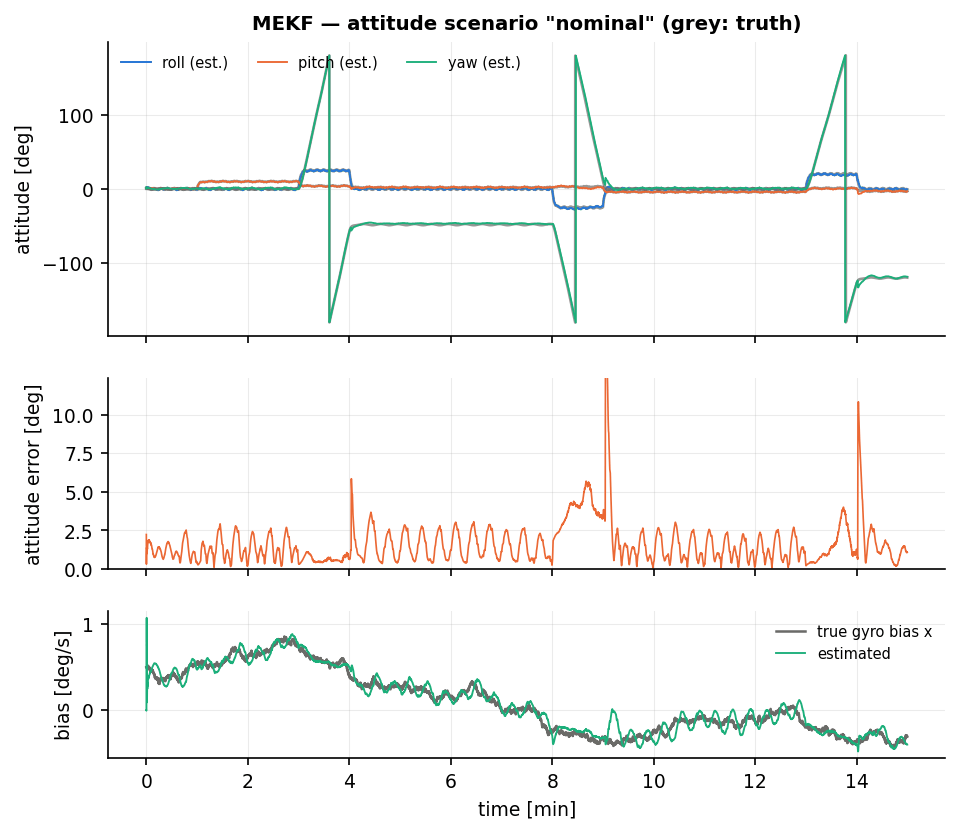
\includegraphics[width=\textwidth]{figures/imu_MEKF_nominal.png}
\caption{MEKF on the nominal mission: Euler angles, total angular error and the $x$-axis gyro-bias
estimate against truth.}
\end{figure}
\begin{figure}[H]\centering
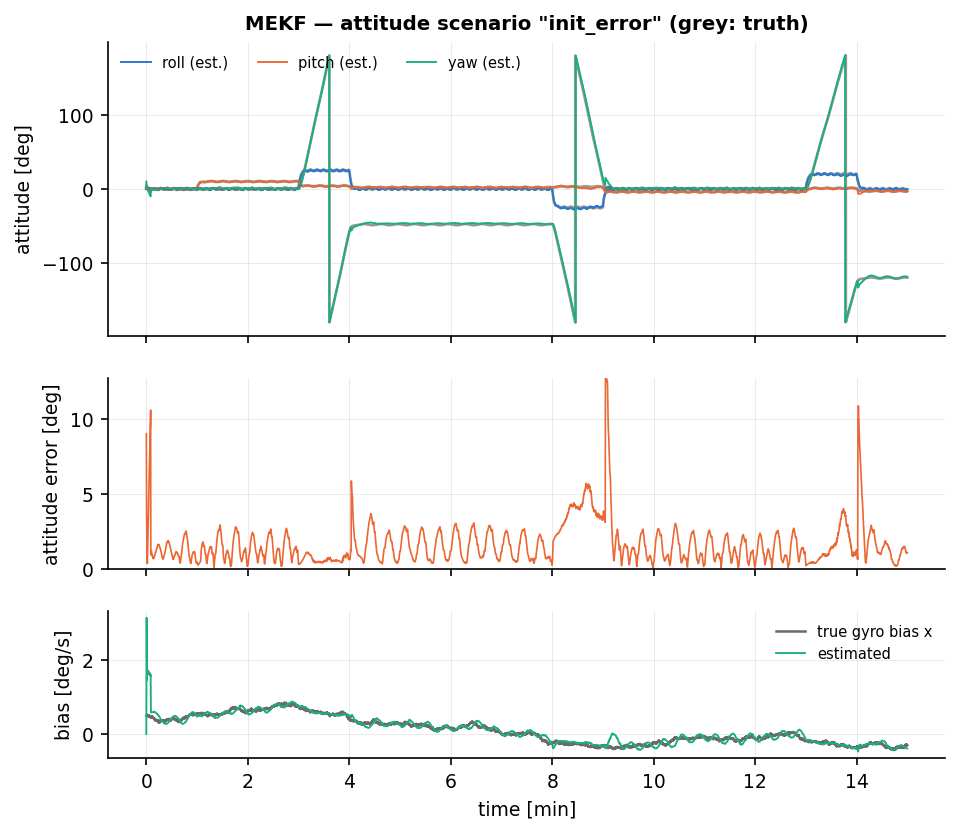
\includegraphics[width=\textwidth]{figures/imu_MEKF_init_error.png}
\caption{MEKF with a $46.6^\circ$ initial attitude error: the transient is over in
$\SI{0.24}{\second}$.}
\end{figure}

The registered MEKF is, with the invariant filter of the next chapter, the most uniform estimator
of the family: mission RMS $2.48/2.50/2.48/2.86/2.14/\SI{3.33}{\degree}$ across the six scenarios in
table order (\texttt{nominal}, \texttt{init\_error}, \texttt{gyro\_bias},
\texttt{mag\_disturbance}, \texttt{vibration}, \texttt{high\_dynamics}); on nominal roll $0.84$,
pitch $0.68$, yaw $\SI{2.23}{\degree}$, $\text{RMS}_{\text{ss}}=\SI{3.07}{\degree}$, peak
$\SI{15.1}{\degree}$, gyro-bias RMSE $\SI{0.17}{\degree\per\second}$ against a true
$\SI{1.03}{\degree\per\second}$, never lost, $t_{\text{conv}}=\SI{0}{\second}$,
$\SI{2.04}{\micro\second}$/step. The flatness of that row is the headline: the six-state filter is
essentially \emph{insensitive} to which scenario it is run on, which is what a correct covariance is
for. It is no longer the outright best --- \texttt{Mahony-Gated} (Chapter~\ref{ch:att-mahony})
reaches $\SI{2.14}{\degree}$ on nominal at one fifteenth of the cost --- but it is the only filter
apart from its invariant twin that is within $\SI{1}{\degree}$ of its own best on every scenario.

Table numbers are three-seed means; the ablations below are single-seed (seed~1) diagnostics, for
which the registered configuration scores $\SI{2.11}{\degree}$ on \texttt{nominal}.

\paragraph{Where the remaining $\SI{2.5}{\degree}$ lives.} Per phase on nominal (seed~1),
\[
1.30\;/\;1.50\;/\;1.15\;/\;1.74\;/\;4.53\;/\;1.91\;/\;2.69\;/\;1.86\ \SI{}{\degree}
\]
for take-off / climb / turn\,1 / cruise / turn\,2 / descent / turn\,3 / final. Two floors, both
quantified independently of any filter:
\begin{itemize}[nosep]
\item \textbf{Hard iron.} The dataset applies an uncompensated body-frame offset
$\bm{b}_m$ with components $0.30$, $-0.15$ and $\SI{0.25}{\micro\tesla}$, i.e.
$\norm{\bm{b}_m}=\SI{0.42}{\micro\tesla}$, or $0.87\,\%$ of the field. (This is the residual of a
\emph{calibrated} compass; the development dataset used $\SI{1.375}{\micro\tesla}$.) Fed to an
\emph{exact} tilt-compensated
compass with the true attitude it alone produces $\SI{0.65}{\degree}$ RMS and $\SI{1.12}{\degree}$
peak of heading error, because the horizontal component of a $65^\circ$-dip field is only
$\SI{20.3}{\micro\tesla}$. No estimator in this family calibrates hard iron~\cite{gebreegziabher2006},
so $\approx\SI{0.65}{\degree}$ of the $\SI{2.23}{\degree}$ yaw RMS is structural; the rest is the
residual tilt error amplified by $\tan I=2.14$.
\item \textbf{Turn coasting.} During the $\SI{60}{\second}$ turns the accelerometer is edited out
and the attitude is carried by the gyro plus the magnetometer alone. At $25^\circ$ of bank the field
lies close to the body vertical (measured: $\bm{m}=[2.0,0.5,47.7]^\T\,\SI{}{\micro\tesla}$ at
$t=\SI{488}{\second}$), so the direction the magnetometer cannot observe --- rotation about the
field --- is close to the heading axis, and the heading is held by the gyro for up to a minute at a
time. The result is $1.15$/$4.53$/$\SI{2.69}{\degree}$ on the three turns, compared with
$42$/$36$/$\SI{35}{\degree}$ for the filters that trust the accelerometer throughout. The second
turn is the worst of the three because it is the longest one flown at constant bank.
\end{itemize}

\paragraph{Ablation of the measurement model.} All on \texttt{nominal}, seed~1:
\begin{center}
\begin{tabular}{@{}lr@{}}
\toprule
configuration & RMS [deg] \\
\midrule
registered & $2.11$ \\
constant $\bm{\Sigma}$ (\code{gate=false}) & $19.61$ \\
magnitude gate only, no manoeuvre bound ($V_{\text{ref}}=0$) & $19.25$ \\
gate + manoeuvre bound but no editing & $7.80$ \\
$\sigma_{a,\text{extra}}=0.1 / 0.5 / \SI{2.0}{\metre\per\second\squared}$ & $4.77 / 2.11 / 1.67$ \\
$\sigma_{m,\text{extra}}=0.3 / 1.5 / \SI{5.0}{\micro\tesla}$ & $2.09 / 2.11 / 2.24$ \\
$q_{\text{scale}}=0.25 / 1 / 4$ & $1.71 / 2.11 / 4.01$ \\
Joseph form off / second-order $\bm{\Phi}$ off & $2.11 / 2.11$ (bit-identical) \\
centripetal mean correction on ($V=45$) & $7.15$ \\
magnetometer disabled & $113.59$ \\
\bottomrule
\end{tabular}
\end{center}
Four readings. First, the magnitude gate on its own is worth \emph{nothing}
($19.25$ versus $19.61$): Remark~\ref{rem:mekf-turn} is not a theoretical point. Second, the
rate-driven bound plus editing is worth a factor of nine, and editing alone is worth
$7.80\to2.11$, i.e. a factor of $3.7$ --- inflating $\bm{\Sigma}$ is not the same as rejecting the
measurement. Third, the filter is now essentially insensitive to
$\sigma_{m,\text{extra}}$ on nominal ($2.09$--$\SI{2.24}{\degree}$ over a factor of 17), which is
what one expects once the hard iron has been calibrated down to $\SI{0.42}{\micro\tesla}$; the one
place it still matters is \texttt{init\_error}, where $\sigma_{m,\text{extra}}=\SI{0.3}{\micro\tesla}$
costs $\SI{4.78}{\degree}$ against $\SI{2.16}{}$, because an over-confident magnetometer pulls the
filter too hard during the initial transient. Fourth, and least expected: switching on the
centripetal \emph{mean} correction --- which is what rescues the fixed-gain filter of
Chapter~\ref{ch:att-complementary} --- makes the MEKF \emph{worse}, $7.15$ against
$\SI{2.11}{\degree}$, and quadruples the bias RMSE ($0.68$ against
$\SI{0.17}{\degree\per\second}$). The reason is structural: the correction
$\bm{f}-(\bm{\omega}_y-\hat{\bm{b}})\times\bm{v}_b$ makes the \emph{measurement} a function of the
\emph{state estimate}, so a bias error can be explained away as a tilt error and vice versa. The
filter loses bias observability, which is precisely the state the MEKF exists to estimate. A
covariance-carrying filter should widen $\bm{\Sigma}$, not modify $\bm{y}$.

\paragraph{Initial-error transient.} From $46.6^\circ$ of attitude error the MEKF is below $5^\circ$
in $\SI{0.17}{\second}$ (17 samples) and below $2^\circ$ in $\SI{0.61}{\second}$; the
$\SI{30}{\second}$ window RMS is $\SI{2.71}{\degree}$ against $\SI{1.32}{\degree}$ from a perfect
start. From $78.5^\circ$ it needs $\SI{2.67}{\second}$ and the window RMS rises to
$\SI{3.52}{\degree}$: the first-order expansion
\eqref{eq:mekf-dtheta}--\eqref{eq:mekf-H} is being pushed past its validity, and the filter spends
the first two seconds correcting in a slightly wrong direction. The cost is visible even in the
table: on \texttt{init\_error} the MEKF's $t_{\text{conv}}$ slips to $\SI{3}{\second}$ and its bias
RMSE to $\SI{0.25}{\degree\per\second}$, against $\SI{0}{\second}$ and $\SI{0.18}{}$ for the
invariant filter. That degradation is exactly what the invariant formulation of
Chapter~\ref{ch:att-iekf} removes.

\paragraph{Cross-scenario detail.} \texttt{vibration} is the \emph{best} scenario
($\SI{2.14}{\degree}$): the configured $\sigma_a$ rises from $0.05$ to
$\SI{1.05}{\metre\per\second\squared}$, the filter widens $\bm{\Sigma}_a$ accordingly and simply
averages more --- this is the textbook demonstration of what a covariance-weighted filter buys over
a fixed-gain one (Madgwick: $14.78$, Mahony: $\SI{18.28}{\degree}$ on the same data).
\texttt{mag\_disturbance} costs $\SI{0.38}{\degree}$, all of it in yaw ($2.23\to2.64$): the field
magnitude rises from $48$ to $\SI{54}{\micro\tesla}$, $e_m$ exceeds the editing threshold and the
magnetometer is dropped for the $\SI{20}{\second}$ of the anomaly, during which the heading is held
by the gyro (cruise-phase RMS $1.74\to\SI{3.06}{\degree}$, seed~1). \texttt{gyro\_bias} costs
$\SI{0.004}{\degree}$ and the bias RMSE only rises from $0.17$ to $\SI{0.19}{\degree\per\second}$.
\texttt{high\_dynamics} is the worst at $\SI{3.33}{\degree}$ with
$t_{\text{conv}}=\SI{222}{\second}$, because the tripled turbulence rates cross the manoeuvre
threshold more often and the accelerometer is edited out more of the time.

\section{Summary}
The MEKF is the reference solution and behaves like one: $\SI{2.5}{\degree}$ RMS, flat to within
$\SI{1.2}{\degree}$ across all six scenarios, $\SI{0.17}{\degree\per\second}$ of bias error, never
lost, $\SI{2.04}{\micro\second}$ and 608\,bytes. Use it whenever a covariance is wanted downstream,
whenever the sensor statistics change during the mission (\texttt{vibration} is
$\SI{2.1}{\degree}$ here against $\SI{18.3}{\degree}$ for the published fixed-gain filters), and
whenever the gyro bias matters. Note, though, that a $\SI{132}{\nano\second}$ nonlinear observer
with the same disturbance model (\texttt{Mahony-Gated}) beats it on \texttt{nominal}
($2.14$ against $2.48$) and \texttt{mag\_disturbance} ($2.31$ against $\SI{2.86}{\degree}$): the
covariance earns its keep on the four \emph{hard} scenarios --- \texttt{init\_error}
($2.50$ against $3.76$), \texttt{gyro\_bias} ($2.48$ against $2.74$), \texttt{vibration}
($2.14$ against $2.47$) and \texttt{high\_dynamics} ($3.33$ against $\SI{4.83}{\degree}$) --- and in
the uncertainty it reports, not in the nominal RMS. The two things
to get right are not in the Kalman equations at all: the per-sample to per-root-second conversion
\eqref{eq:mekf-units}, and a measurement-covariance model that can see a coordinated turn
(Remark~\ref{rem:mekf-turn}) and edit it out rather than average it in. Its one structural weakness
--- a first-order error expansion that degrades above $\approx60^\circ$ of initial error --- is the
subject of the next chapter.
